\documentclass{standalone}
\usepackage{tikz}
\usetikzlibrary{patterns, positioning}


\begin{document}
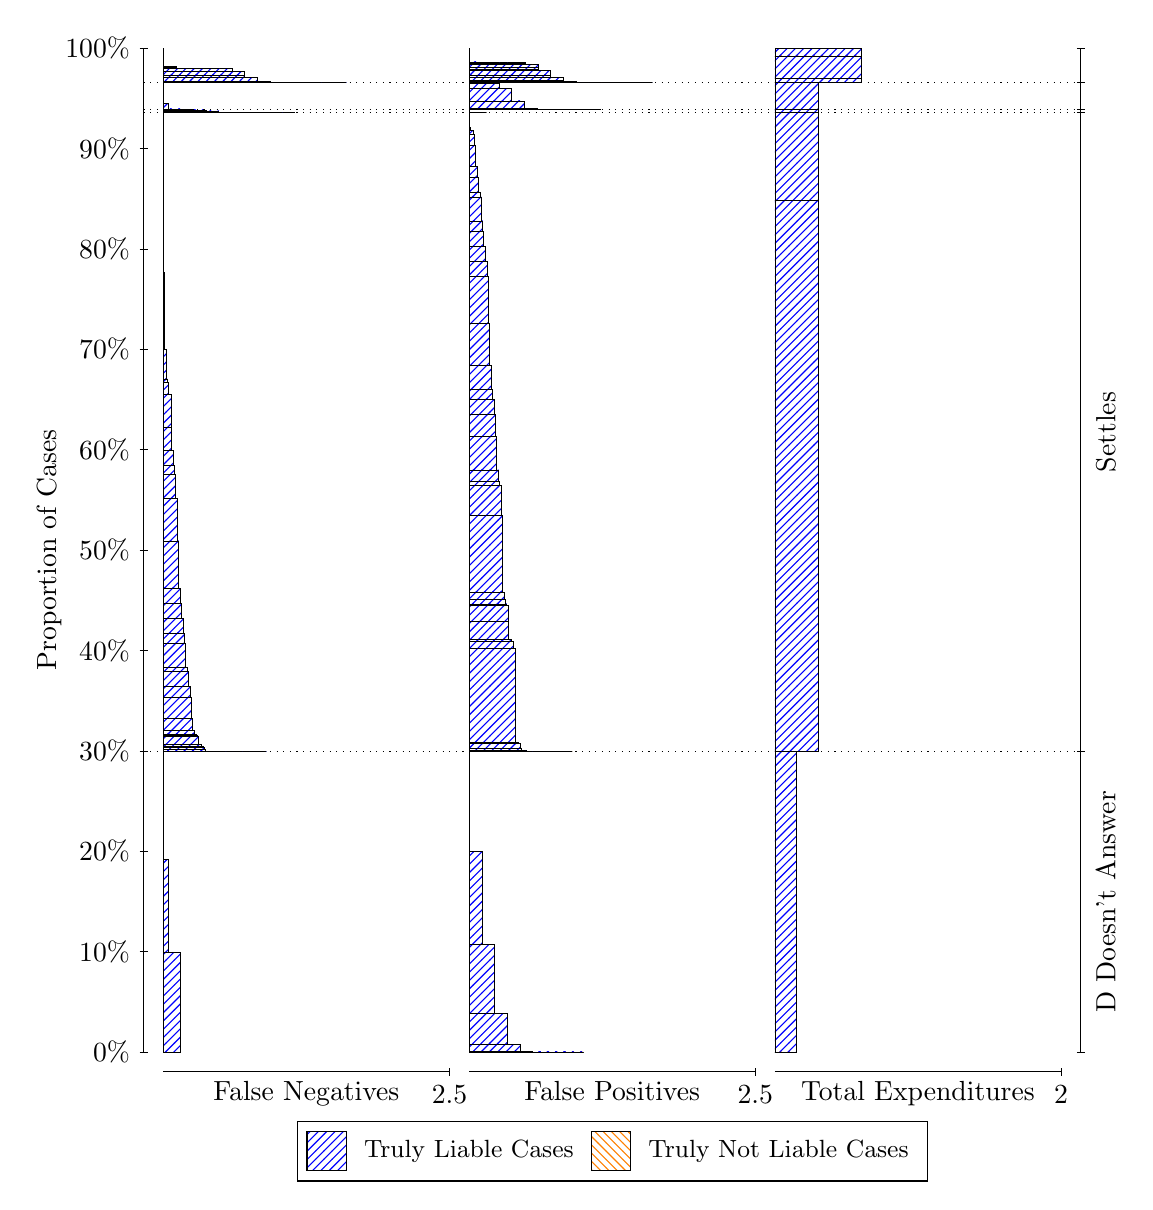
\begin{tikzpicture}
\draw[black, very thin] (1.5,1.75) -- (1.5,14.5);
\node[rotate=90, text=black, anchor=center] at (0.3, 8.125) {Proportion of Cases};
\draw[black, very thin] (1.45,1.75) -- (1.55,1.75);
\node[text=black, anchor=east] at (1.45, 1.75) {0\%};
\draw[black, very thin] (1.45,3.025) -- (1.55,3.025);
\node[text=black, anchor=east] at (1.45, 3.025) {10\%};
\draw[black, very thin] (1.45,4.3) -- (1.55,4.3);
\node[text=black, anchor=east] at (1.45, 4.3) {20\%};
\draw[black, very thin] (1.45,5.575) -- (1.55,5.575);
\node[text=black, anchor=east] at (1.45, 5.575) {30\%};
\draw[black, very thin] (1.45,6.85) -- (1.55,6.85);
\node[text=black, anchor=east] at (1.45, 6.85) {40\%};
\draw[black, very thin] (1.45,8.125) -- (1.55,8.125);
\node[text=black, anchor=east] at (1.45, 8.125) {50\%};
\draw[black, very thin] (1.45,9.4) -- (1.55,9.4);
\node[text=black, anchor=east] at (1.45, 9.4) {60\%};
\draw[black, very thin] (1.45,10.675) -- (1.55,10.675);
\node[text=black, anchor=east] at (1.45, 10.675) {70\%};
\draw[black, very thin] (1.45,11.95) -- (1.55,11.95);
\node[text=black, anchor=east] at (1.45, 11.95) {80\%};
\draw[black, very thin] (1.45,13.225) -- (1.55,13.225);
\node[text=black, anchor=east] at (1.45, 13.225) {90\%};
\draw[black, very thin] (1.45,14.5) -- (1.55,14.5);
\node[text=black, anchor=east] at (1.45, 14.5) {100\%};

\draw[black, very thin] (13.4,1.75) -- (13.4,14.5);
\draw[black, very thin] (13.35,1.75) -- (13.45,1.75);
\node[anchor=west] at (13.35, 1.75) {};
\draw[black, very thin] (13.35,5.5631) -- (13.45,5.5631);
\node[anchor=west] at (13.35, 5.5631) {};
\draw[black, very thin] (13.35,13.681) -- (13.45,13.681);
\node[anchor=west] at (13.35, 13.681) {};
\draw[black, very thin] (13.35,13.718) -- (13.45,13.718);
\node[anchor=west] at (13.35, 13.718) {};
\draw[black, very thin] (13.35,14.06) -- (13.45,14.06);
\node[anchor=west] at (13.35, 14.06) {};
\draw[black, very thin] (13.35,14.5) -- (13.45,14.5);
\node[anchor=west] at (13.35, 14.5) {};

\draw[black, very thin, pattern color=blue, pattern=north east lines] (1.75,1.75) rectangle (1.968,3.0136);
\draw[black, very thin, pattern color=blue, pattern=north east lines] (1.75,3.0136) rectangle (1.8065,4.1973);
\draw[black, very thin, pattern color=orange, pattern=north west lines] (1.75,4.1973) rectangle (1.75,4.1973);
\draw[black, very thin, pattern color=blue, pattern=north east lines] (1.75,4.1973) rectangle (1.75,5.5631);
\draw[black, very thin, pattern color=blue, pattern=north east lines] (1.75,5.5631) rectangle (3.058,5.5631);
\draw[black, very thin, pattern color=blue, pattern=north east lines] (1.75,5.5631) rectangle (2.9853,5.5631);
\draw[black, very thin, pattern color=blue, pattern=north east lines] (1.75,5.5631) rectangle (2.9127,5.5631);
\draw[black, very thin, pattern color=blue, pattern=north east lines] (1.75,5.5631) rectangle (2.8965,5.5631);
\draw[black, very thin, pattern color=blue, pattern=north east lines] (1.75,5.5631) rectangle (2.84,5.5631);
\draw[black, very thin, pattern color=blue, pattern=north east lines] (1.75,5.5631) rectangle (2.8239,5.5631);
\draw[black, very thin, pattern color=blue, pattern=north east lines] (1.75,5.5631) rectangle (2.7673,5.5631);
\draw[black, very thin, pattern color=blue, pattern=north east lines] (1.75,5.5631) rectangle (2.7512,5.5631);
\draw[black, very thin, pattern color=blue, pattern=north east lines] (1.75,5.5631) rectangle (2.735,5.5631);
\draw[black, very thin, pattern color=blue, pattern=north east lines] (1.75,5.5631) rectangle (2.6947,5.5631);
\draw[black, very thin, pattern color=blue, pattern=north east lines] (1.75,5.5631) rectangle (2.6785,5.5631);
\draw[black, very thin, pattern color=blue, pattern=north east lines] (1.75,5.5631) rectangle (2.6624,5.5631);
\draw[black, very thin, pattern color=blue, pattern=north east lines] (1.75,5.5631) rectangle (2.622,5.5631);
\draw[black, very thin, pattern color=blue, pattern=north east lines] (1.75,5.5631) rectangle (2.6059,5.5631);
\draw[black, very thin, pattern color=blue, pattern=north east lines] (1.75,5.5631) rectangle (2.5897,5.5631);
\draw[black, very thin, pattern color=blue, pattern=north east lines] (1.75,5.5631) rectangle (2.5736,5.5631);
\draw[black, very thin, pattern color=blue, pattern=north east lines] (1.75,5.5631) rectangle (2.5493,5.5631);
\draw[black, very thin, pattern color=blue, pattern=north east lines] (1.75,5.5631) rectangle (2.5332,5.5631);
\draw[black, very thin, pattern color=blue, pattern=north east lines] (1.75,5.5631) rectangle (2.517,5.5631);
\draw[black, very thin, pattern color=blue, pattern=north east lines] (1.75,5.5631) rectangle (2.5009,5.5631);
\draw[black, very thin, pattern color=blue, pattern=north east lines] (1.75,5.5631) rectangle (2.4605,5.5631);
\draw[black, very thin, pattern color=blue, pattern=north east lines] (1.75,5.5631) rectangle (2.4444,5.5636);
\draw[black, very thin, pattern color=blue, pattern=north east lines] (1.75,5.5636) rectangle (2.4282,5.5642);
\draw[black, very thin, pattern color=blue, pattern=north east lines] (1.75,5.5642) rectangle (2.4121,5.5644);
\draw[black, very thin, pattern color=blue, pattern=north east lines] (1.75,5.5644) rectangle (2.3879,5.565);
\draw[black, very thin, pattern color=blue, pattern=north east lines] (1.75,5.565) rectangle (2.3717,5.5651);
\draw[black, very thin, pattern color=blue, pattern=north east lines] (1.75,5.5651) rectangle (2.3556,5.5702);
\draw[black, very thin, pattern color=blue, pattern=north east lines] (1.75,5.5702) rectangle (2.3394,5.5705);
\draw[black, very thin, pattern color=blue, pattern=north east lines] (1.75,5.5705) rectangle (2.3313,5.5712);
\draw[black, very thin, pattern color=blue, pattern=north east lines] (1.75,5.5712) rectangle (2.299,5.5736);
\draw[black, very thin, pattern color=blue, pattern=north east lines] (1.75,5.5736) rectangle (2.2829,5.5941);
\draw[black, very thin, pattern color=blue, pattern=north east lines] (1.75,5.5941) rectangle (2.2667,5.621);
\draw[black, very thin, pattern color=blue, pattern=north east lines] (1.75,5.621) rectangle (2.2506,5.6325);
\draw[black, very thin, pattern color=blue, pattern=north east lines] (1.75,5.6325) rectangle (2.2264,5.6561);
\draw[black, very thin, pattern color=blue, pattern=north east lines] (1.75,5.6561) rectangle (2.2102,5.6611);
\draw[black, very thin, pattern color=blue, pattern=north east lines] (1.75,5.6611) rectangle (2.1941,5.7543);
\draw[black, very thin, pattern color=blue, pattern=north east lines] (1.75,5.7543) rectangle (2.1779,5.769);
\draw[black, very thin, pattern color=blue, pattern=north east lines] (1.75,5.769) rectangle (2.1699,5.7896);
\draw[black, very thin, pattern color=blue, pattern=north east lines] (1.75,5.7896) rectangle (2.1376,5.8379);
\draw[black, very thin, pattern color=blue, pattern=north east lines] (1.75,5.8379) rectangle (2.1214,5.9855);
\draw[black, very thin, pattern color=blue, pattern=north east lines] (1.75,5.9855) rectangle (2.1053,6.2496);
\draw[black, very thin, pattern color=blue, pattern=north east lines] (1.75,6.2496) rectangle (2.0891,6.3891);
\draw[black, very thin, pattern color=blue, pattern=north east lines] (1.75,6.3891) rectangle (2.0649,6.5818);
\draw[black, very thin, pattern color=blue, pattern=north east lines] (1.75,6.5818) rectangle (2.0487,6.635);
\draw[black, very thin, pattern color=blue, pattern=north east lines] (1.75,6.635) rectangle (2.0326,6.9399);
\draw[black, very thin, pattern color=blue, pattern=north east lines] (1.75,6.9399) rectangle (2.0164,7.0722);
\draw[black, very thin, pattern color=blue, pattern=north east lines] (1.75,7.0722) rectangle (2.0084,7.2593);
\draw[black, very thin, pattern color=blue, pattern=north east lines] (1.75,7.2593) rectangle (1.9761,7.4518);
\draw[black, very thin, pattern color=blue, pattern=north east lines] (1.75,7.4518) rectangle (1.9599,7.6443);
\draw[black, very thin, pattern color=blue, pattern=north east lines] (1.75,7.6443) rectangle (1.9438,8.2413);
\draw[black, very thin, pattern color=blue, pattern=north east lines] (1.75,8.2413) rectangle (1.9276,8.7771);
\draw[black, very thin, pattern color=blue, pattern=north east lines] (1.75,8.7771) rectangle (1.9034,9.082);
\draw[black, very thin, pattern color=blue, pattern=north east lines] (1.75,9.082) rectangle (1.8873,9.201);
\draw[black, very thin, pattern color=blue, pattern=north east lines] (1.75,9.201) rectangle (1.8711,9.3936);
\draw[black, very thin, pattern color=blue, pattern=north east lines] (1.75,9.3936) rectangle (1.855,9.6779);
\draw[black, very thin, pattern color=blue, pattern=north east lines] (1.75,9.6779) rectangle (1.8469,10.103);
\draw[black, very thin, pattern color=blue, pattern=north east lines] (1.75,10.103) rectangle (1.8146,10.25);
\draw[black, very thin, pattern color=blue, pattern=north east lines] (1.75,10.25) rectangle (1.7984,10.298);
\draw[black, very thin, pattern color=blue, pattern=north east lines] (1.75,10.298) rectangle (1.7823,10.679);
\draw[black, very thin, pattern color=blue, pattern=north east lines] (1.75,10.679) rectangle (1.7661,11.651);
\draw[black, very thin, pattern color=orange, pattern=north west lines] (1.75,11.651) rectangle (1.75,11.651);
\draw[black, very thin, pattern color=blue, pattern=north east lines] (1.75,11.651) rectangle (1.75,13.681);
\draw[black, very thin, pattern color=blue, pattern=north east lines] (1.75,13.681) rectangle (3.4213,13.681);
\draw[black, very thin, pattern color=blue, pattern=north east lines] (1.75,13.681) rectangle (3.2599,13.681);
\draw[black, very thin, pattern color=blue, pattern=north east lines] (1.75,13.681) rectangle (3.0984,13.681);
\draw[black, very thin, pattern color=blue, pattern=north east lines] (1.75,13.681) rectangle (2.9369,13.681);
\draw[black, very thin, pattern color=blue, pattern=north east lines] (1.75,13.681) rectangle (2.7754,13.681);
\draw[black, very thin, pattern color=blue, pattern=north east lines] (1.75,13.681) rectangle (2.6139,13.686);
\draw[black, very thin, pattern color=blue, pattern=north east lines] (1.75,13.686) rectangle (2.4524,13.703);
\draw[black, very thin, pattern color=blue, pattern=north east lines] (1.75,13.703) rectangle (2.291,13.715);
\draw[black, very thin, pattern color=blue, pattern=north east lines] (1.75,13.715) rectangle (2.1295,13.717);
\draw[black, very thin, pattern color=blue, pattern=north east lines] (1.75,13.717) rectangle (1.968,13.718);
\draw[black, very thin, pattern color=orange, pattern=north west lines] (1.75,13.718) rectangle (1.75,13.718);
\draw[black, very thin, pattern color=blue, pattern=north east lines] (1.75,13.718) rectangle (1.968,13.728);
\draw[black, very thin, pattern color=blue, pattern=north east lines] (1.75,13.728) rectangle (1.8065,13.794);
\draw[black, very thin, pattern color=orange, pattern=north west lines] (1.75,13.794) rectangle (1.75,13.794);
\draw[black, very thin, pattern color=blue, pattern=north east lines] (1.75,13.794) rectangle (1.75,14.06);
\draw[black, very thin, pattern color=blue, pattern=north east lines] (1.75,14.06) rectangle (4.0753,14.06);
\draw[black, very thin, pattern color=blue, pattern=north east lines] (1.75,14.06) rectangle (3.9139,14.06);
\draw[black, very thin, pattern color=blue, pattern=north east lines] (1.75,14.06) rectangle (3.7524,14.06);
\draw[black, very thin, pattern color=blue, pattern=north east lines] (1.75,14.06) rectangle (3.5909,14.06);
\draw[black, very thin, pattern color=blue, pattern=north east lines] (1.75,14.06) rectangle (3.4294,14.061);
\draw[black, very thin, pattern color=blue, pattern=north east lines] (1.75,14.061) rectangle (3.2679,14.062);
\draw[black, very thin, pattern color=blue, pattern=north east lines] (1.75,14.062) rectangle (3.2679,14.064);
\draw[black, very thin, pattern color=blue, pattern=north east lines] (1.75,14.064) rectangle (3.1064,14.079);
\draw[black, very thin, pattern color=blue, pattern=north east lines] (1.75,14.079) rectangle (3.1064,14.079);
\draw[black, very thin, pattern color=blue, pattern=north east lines] (1.75,14.079) rectangle (2.945,14.127);
\draw[black, very thin, pattern color=blue, pattern=north east lines] (1.75,14.127) rectangle (2.7835,14.158);
\draw[black, very thin, pattern color=blue, pattern=north east lines] (1.75,14.158) rectangle (2.7835,14.2);
\draw[black, very thin, pattern color=blue, pattern=north east lines] (1.75,14.2) rectangle (2.7189,14.2);
\draw[black, very thin, pattern color=blue, pattern=north east lines] (1.75,14.2) rectangle (2.622,14.238);
\draw[black, very thin, pattern color=blue, pattern=north east lines] (1.75,14.238) rectangle (2.5574,14.238);
\draw[black, very thin, pattern color=blue, pattern=north east lines] (1.75,14.238) rectangle (2.4605,14.239);
\draw[black, very thin, pattern color=blue, pattern=north east lines] (1.75,14.239) rectangle (2.4605,14.242);
\draw[black, very thin, pattern color=blue, pattern=north east lines] (1.75,14.242) rectangle (2.4605,14.242);
\draw[black, very thin, pattern color=blue, pattern=north east lines] (1.75,14.242) rectangle (2.3959,14.242);
\draw[black, very thin, pattern color=blue, pattern=north east lines] (1.75,14.242) rectangle (2.3959,14.242);
\draw[black, very thin, pattern color=blue, pattern=north east lines] (1.75,14.242) rectangle (2.299,14.242);
\draw[black, very thin, pattern color=blue, pattern=north east lines] (1.75,14.242) rectangle (2.299,14.242);
\draw[black, very thin, pattern color=blue, pattern=north east lines] (1.75,14.242) rectangle (2.2344,14.242);
\draw[black, very thin, pattern color=blue, pattern=north east lines] (1.75,14.242) rectangle (2.2344,14.242);
\draw[black, very thin, pattern color=blue, pattern=north east lines] (1.75,14.242) rectangle (2.2344,14.242);
\draw[black, very thin, pattern color=blue, pattern=north east lines] (1.75,14.242) rectangle (2.1376,14.242);
\draw[black, very thin, pattern color=blue, pattern=north east lines] (1.75,14.242) rectangle (2.1376,14.242);
\draw[black, very thin, pattern color=blue, pattern=north east lines] (1.75,14.242) rectangle (2.073,14.243);
\draw[black, very thin, pattern color=blue, pattern=north east lines] (1.75,14.243) rectangle (2.073,14.244);
\draw[black, very thin, pattern color=blue, pattern=north east lines] (1.75,14.244) rectangle (1.9761,14.244);
\draw[black, very thin, pattern color=blue, pattern=north east lines] (1.75,14.244) rectangle (1.9761,14.244);
\draw[black, very thin, pattern color=blue, pattern=north east lines] (1.75,14.244) rectangle (1.9115,14.247);
\draw[black, very thin, pattern color=blue, pattern=north east lines] (1.75,14.247) rectangle (1.9115,14.251);
\draw[black, very thin, pattern color=blue, pattern=north east lines] (1.75,14.251) rectangle (1.9115,14.265);
\draw[black, very thin, pattern color=blue, pattern=north east lines] (1.75,14.265) rectangle (1.8146,14.265);
\draw[black, very thin, pattern color=blue, pattern=north east lines] (1.75,14.265) rectangle (1.8146,14.265);
\draw[black, very thin, pattern color=orange, pattern=north west lines] (1.75,14.265) rectangle (1.75,14.265);
\draw[black, very thin, pattern color=blue, pattern=north east lines] (1.75,14.265) rectangle (1.75,14.5);
\draw[black, very thin, pattern color=orange, pattern=north west lines] (5.6333,1.75) rectangle (7.0867,1.75);
\draw[black, very thin, pattern color=blue, pattern=north east lines] (5.6333,1.75) rectangle (7.0867,1.75);
\draw[black, very thin, pattern color=blue, pattern=north east lines] (5.6333,1.75) rectangle (6.9252,1.75);
\draw[black, very thin, pattern color=blue, pattern=north east lines] (5.6333,1.75) rectangle (6.7637,1.75);
\draw[black, very thin, pattern color=blue, pattern=north east lines] (5.6333,1.75) rectangle (6.6022,1.7503);
\draw[black, very thin, pattern color=blue, pattern=north east lines] (5.6333,1.7503) rectangle (6.4407,1.7582);
\draw[black, very thin, pattern color=blue, pattern=north east lines] (5.6333,1.7582) rectangle (6.2793,1.8434);
\draw[black, very thin, pattern color=blue, pattern=north east lines] (5.6333,1.8434) rectangle (6.1178,2.2366);
\draw[black, very thin, pattern color=blue, pattern=north east lines] (5.6333,2.2366) rectangle (5.9563,3.1157);
\draw[black, very thin, pattern color=blue, pattern=north east lines] (5.6333,3.1157) rectangle (5.7948,4.2995);
\draw[black, very thin, pattern color=blue, pattern=north east lines] (5.6333,4.2995) rectangle (5.6333,5.5631);
\draw[black, very thin, pattern color=orange, pattern=north west lines] (5.6333,5.5631) rectangle (6.9413,5.5631);
\draw[black, very thin, pattern color=blue, pattern=north east lines] (5.6333,5.5631) rectangle (6.9413,5.5631);
\draw[black, very thin, pattern color=blue, pattern=north east lines] (5.6333,5.5631) rectangle (6.7799,5.5631);
\draw[black, very thin, pattern color=orange, pattern=north west lines] (5.6333,5.5631) rectangle (6.7233,5.5631);
\draw[black, very thin, pattern color=blue, pattern=north east lines] (5.6333,5.5631) rectangle (6.7233,5.5631);
\draw[black, very thin, pattern color=orange, pattern=north west lines] (5.6333,5.5631) rectangle (6.6507,5.5631);
\draw[black, very thin, pattern color=blue, pattern=north east lines] (5.6333,5.5631) rectangle (6.6507,5.5631);
\draw[black, very thin, pattern color=blue, pattern=north east lines] (5.6333,5.5631) rectangle (6.6184,5.5631);
\draw[black, very thin, pattern color=orange, pattern=north west lines] (5.6333,5.5631) rectangle (6.578,5.5631);
\draw[black, very thin, pattern color=blue, pattern=north east lines] (5.6333,5.5631) rectangle (6.578,5.5631);
\draw[black, very thin, pattern color=blue, pattern=north east lines] (5.6333,5.5631) rectangle (6.5619,5.5631);
\draw[black, very thin, pattern color=orange, pattern=north west lines] (5.6333,5.5631) rectangle (6.5053,5.5631);
\draw[black, very thin, pattern color=blue, pattern=north east lines] (5.6333,5.5631) rectangle (6.5053,5.5631);
\draw[black, very thin, pattern color=blue, pattern=north east lines] (5.6333,5.5631) rectangle (6.4892,5.5631);
\draw[black, very thin, pattern color=blue, pattern=north east lines] (5.6333,5.5631) rectangle (6.4569,5.5636);
\draw[black, very thin, pattern color=orange, pattern=north west lines] (5.6333,5.5636) rectangle (6.4327,5.5636);
\draw[black, very thin, pattern color=blue, pattern=north east lines] (5.6333,5.5636) rectangle (6.4327,5.5636);
\draw[black, very thin, pattern color=blue, pattern=north east lines] (5.6333,5.5636) rectangle (6.4165,5.5639);
\draw[black, very thin, pattern color=blue, pattern=north east lines] (5.6333,5.5639) rectangle (6.4004,5.564);
\draw[black, very thin, pattern color=orange, pattern=north west lines] (5.6333,5.564) rectangle (6.36,5.564);
\draw[black, very thin, pattern color=blue, pattern=north east lines] (5.6333,5.564) rectangle (6.36,5.5754);
\draw[black, very thin, pattern color=blue, pattern=north east lines] (5.6333,5.5754) rectangle (6.3439,5.5754);
\draw[black, very thin, pattern color=blue, pattern=north east lines] (5.6333,5.5754) rectangle (6.3277,5.5759);
\draw[black, very thin, pattern color=blue, pattern=north east lines] (5.6333,5.5759) rectangle (6.2954,5.6007);
\draw[black, very thin, pattern color=orange, pattern=north west lines] (5.6333,5.6007) rectangle (6.2873,5.6007);
\draw[black, very thin, pattern color=blue, pattern=north east lines] (5.6333,5.6007) rectangle (6.2873,5.67);
\draw[black, very thin, pattern color=blue, pattern=north east lines] (5.6333,5.67) rectangle (6.2712,5.6706);
\draw[black, very thin, pattern color=blue, pattern=north east lines] (5.6333,5.6706) rectangle (6.255,5.678);
\draw[black, very thin, pattern color=blue, pattern=north east lines] (5.6333,5.678) rectangle (6.2389,5.6832);
\draw[black, very thin, pattern color=orange, pattern=north west lines] (5.6333,5.6832) rectangle (6.2147,5.6832);
\draw[black, very thin, pattern color=blue, pattern=north east lines] (5.6333,5.6832) rectangle (6.2147,6.877);
\draw[black, very thin, pattern color=blue, pattern=north east lines] (5.6333,6.877) rectangle (6.1985,6.9687);
\draw[black, very thin, pattern color=blue, pattern=north east lines] (5.6333,6.9687) rectangle (6.1824,6.971);
\draw[black, very thin, pattern color=blue, pattern=north east lines] (5.6333,6.971) rectangle (6.1662,6.9915);
\draw[black, very thin, pattern color=blue, pattern=north east lines] (5.6333,6.9915) rectangle (6.1339,7.214);
\draw[black, very thin, pattern color=blue, pattern=north east lines] (5.6333,7.214) rectangle (6.1259,7.4176);
\draw[black, very thin, pattern color=blue, pattern=north east lines] (5.6333,7.4176) rectangle (6.1097,7.4412);
\draw[black, very thin, pattern color=blue, pattern=north east lines] (5.6333,7.4412) rectangle (6.0936,7.4999);
\draw[black, very thin, pattern color=blue, pattern=north east lines] (5.6333,7.4999) rectangle (6.0774,7.5931);
\draw[black, very thin, pattern color=blue, pattern=north east lines] (5.6333,7.5931) rectangle (6.0532,8.5654);
\draw[black, very thin, pattern color=blue, pattern=north east lines] (5.6333,8.5654) rectangle (6.037,8.9458);
\draw[black, very thin, pattern color=blue, pattern=north east lines] (5.6333,8.9458) rectangle (6.0209,8.994);
\draw[black, very thin, pattern color=blue, pattern=north east lines] (5.6333,8.994) rectangle (6.0047,9.1416);
\draw[black, very thin, pattern color=blue, pattern=north east lines] (5.6333,9.1416) rectangle (5.9724,9.5663);
\draw[black, very thin, pattern color=blue, pattern=north east lines] (5.6333,9.5663) rectangle (5.9644,9.8506);
\draw[black, very thin, pattern color=blue, pattern=north east lines] (5.6333,9.8506) rectangle (5.9482,10.043);
\draw[black, very thin, pattern color=blue, pattern=north east lines] (5.6333,10.043) rectangle (5.9321,10.162);
\draw[black, very thin, pattern color=blue, pattern=north east lines] (5.6333,10.162) rectangle (5.9159,10.467);
\draw[black, very thin, pattern color=blue, pattern=north east lines] (5.6333,10.467) rectangle (5.8917,11.003);
\draw[black, very thin, pattern color=blue, pattern=north east lines] (5.6333,11.003) rectangle (5.8756,11.6);
\draw[black, very thin, pattern color=blue, pattern=north east lines] (5.6333,11.6) rectangle (5.8594,11.792);
\draw[black, very thin, pattern color=blue, pattern=north east lines] (5.6333,11.792) rectangle (5.8433,11.985);
\draw[black, very thin, pattern color=blue, pattern=north east lines] (5.6333,11.985) rectangle (5.811,12.172);
\draw[black, very thin, pattern color=blue, pattern=north east lines] (5.6333,12.172) rectangle (5.8029,12.304);
\draw[black, very thin, pattern color=blue, pattern=north east lines] (5.6333,12.304) rectangle (5.7867,12.609);
\draw[black, very thin, pattern color=blue, pattern=north east lines] (5.6333,12.609) rectangle (5.7706,12.662);
\draw[black, very thin, pattern color=blue, pattern=north east lines] (5.6333,12.662) rectangle (5.7544,12.855);
\draw[black, very thin, pattern color=blue, pattern=north east lines] (5.6333,12.855) rectangle (5.7302,12.995);
\draw[black, very thin, pattern color=blue, pattern=north east lines] (5.6333,12.995) rectangle (5.7141,13.259);
\draw[black, very thin, pattern color=blue, pattern=north east lines] (5.6333,13.259) rectangle (5.6979,13.406);
\draw[black, very thin, pattern color=blue, pattern=north east lines] (5.6333,13.406) rectangle (5.6818,13.455);
\draw[black, very thin, pattern color=blue, pattern=north east lines] (5.6333,13.455) rectangle (5.6495,13.475);
\draw[black, very thin, pattern color=blue, pattern=north east lines] (5.6333,13.475) rectangle (5.6414,13.49);
\draw[black, very thin, pattern color=blue, pattern=north east lines] (5.6333,13.49) rectangle (5.6333,13.681);
\draw[black, very thin, pattern color=orange, pattern=north west lines] (5.6333,13.681) rectangle (5.8513,13.681);
\draw[black, very thin, pattern color=blue, pattern=north east lines] (5.6333,13.681) rectangle (5.8513,13.681);
\draw[black, very thin, pattern color=blue, pattern=north east lines] (5.6333,13.681) rectangle (5.6899,13.683);
\draw[black, very thin, pattern color=blue, pattern=north east lines] (5.6333,13.683) rectangle (5.6333,13.718);
\draw[black, very thin, pattern color=orange, pattern=north west lines] (5.6333,13.718) rectangle (7.3047,13.718);
\draw[black, very thin, pattern color=blue, pattern=north east lines] (5.6333,13.718) rectangle (7.3047,13.718);
\draw[black, very thin, pattern color=blue, pattern=north east lines] (5.6333,13.718) rectangle (7.1432,13.718);
\draw[black, very thin, pattern color=blue, pattern=north east lines] (5.6333,13.718) rectangle (6.9817,13.718);
\draw[black, very thin, pattern color=blue, pattern=north east lines] (5.6333,13.718) rectangle (6.8202,13.718);
\draw[black, very thin, pattern color=blue, pattern=north east lines] (5.6333,13.718) rectangle (6.6587,13.718);
\draw[black, very thin, pattern color=blue, pattern=north east lines] (5.6333,13.718) rectangle (6.4973,13.733);
\draw[black, very thin, pattern color=blue, pattern=north east lines] (5.6333,13.733) rectangle (6.3358,13.83);
\draw[black, very thin, pattern color=blue, pattern=north east lines] (5.6333,13.83) rectangle (6.1743,13.984);
\draw[black, very thin, pattern color=blue, pattern=north east lines] (5.6333,13.984) rectangle (6.0128,14.05);
\draw[black, very thin, pattern color=blue, pattern=north east lines] (5.6333,14.05) rectangle (5.8513,14.06);
\draw[black, very thin, pattern color=orange, pattern=north west lines] (5.6333,14.06) rectangle (7.9587,14.06);
\draw[black, very thin, pattern color=blue, pattern=north east lines] (5.6333,14.06) rectangle (7.9587,14.06);
\draw[black, very thin, pattern color=orange, pattern=north west lines] (5.6333,14.06) rectangle (7.7972,14.06);
\draw[black, very thin, pattern color=blue, pattern=north east lines] (5.6333,14.06) rectangle (7.7972,14.06);
\draw[black, very thin, pattern color=orange, pattern=north west lines] (5.6333,14.06) rectangle (7.6357,14.06);
\draw[black, very thin, pattern color=blue, pattern=north east lines] (5.6333,14.06) rectangle (7.6357,14.06);
\draw[black, very thin, pattern color=blue, pattern=north east lines] (5.6333,14.06) rectangle (7.4742,14.06);
\draw[black, very thin, pattern color=orange, pattern=north west lines] (5.6333,14.06) rectangle (7.4742,14.06);
\draw[black, very thin, pattern color=blue, pattern=north east lines] (5.6333,14.06) rectangle (7.4742,14.06);
\draw[black, very thin, pattern color=blue, pattern=north east lines] (5.6333,14.06) rectangle (7.3127,14.06);
\draw[black, very thin, pattern color=orange, pattern=north west lines] (5.6333,14.06) rectangle (7.3127,14.06);
\draw[black, very thin, pattern color=blue, pattern=north east lines] (5.6333,14.06) rectangle (7.3127,14.06);
\draw[black, very thin, pattern color=blue, pattern=north east lines] (5.6333,14.06) rectangle (7.1513,14.063);
\draw[black, very thin, pattern color=orange, pattern=north west lines] (5.6333,14.063) rectangle (7.1513,14.063);
\draw[black, very thin, pattern color=blue, pattern=north east lines] (5.6333,14.063) rectangle (7.1513,14.063);
\draw[black, very thin, pattern color=blue, pattern=north east lines] (5.6333,14.063) rectangle (6.9898,14.067);
\draw[black, very thin, pattern color=orange, pattern=north west lines] (5.6333,14.067) rectangle (6.9898,14.067);
\draw[black, very thin, pattern color=blue, pattern=north east lines] (5.6333,14.067) rectangle (6.9898,14.078);
\draw[black, very thin, pattern color=blue, pattern=north east lines] (5.6333,14.078) rectangle (6.9898,14.079);
\draw[black, very thin, pattern color=blue, pattern=north east lines] (5.6333,14.079) rectangle (6.9898,14.079);
\draw[black, very thin, pattern color=blue, pattern=north east lines] (5.6333,14.079) rectangle (6.8283,14.092);
\draw[black, very thin, pattern color=blue, pattern=north east lines] (5.6333,14.092) rectangle (6.8283,14.124);
\draw[black, very thin, pattern color=blue, pattern=north east lines] (5.6333,14.124) rectangle (6.8283,14.128);
\draw[black, very thin, pattern color=blue, pattern=north east lines] (5.6333,14.128) rectangle (6.6668,14.129);
\draw[black, very thin, pattern color=blue, pattern=north east lines] (5.6333,14.129) rectangle (6.6668,14.16);
\draw[black, very thin, pattern color=blue, pattern=north east lines] (5.6333,14.16) rectangle (6.6668,14.217);
\draw[black, very thin, pattern color=orange, pattern=north west lines] (5.6333,14.217) rectangle (6.6022,14.217);
\draw[black, very thin, pattern color=blue, pattern=north east lines] (5.6333,14.217) rectangle (6.6022,14.217);
\draw[black, very thin, pattern color=blue, pattern=north east lines] (5.6333,14.217) rectangle (6.5053,14.23);
\draw[black, very thin, pattern color=blue, pattern=north east lines] (5.6333,14.23) rectangle (6.5053,14.254);
\draw[black, very thin, pattern color=blue, pattern=north east lines] (5.6333,14.254) rectangle (6.5053,14.296);
\draw[black, very thin, pattern color=orange, pattern=north west lines] (5.6333,14.296) rectangle (6.4407,14.296);
\draw[black, very thin, pattern color=blue, pattern=north east lines] (5.6333,14.296) rectangle (6.4407,14.296);
\draw[black, very thin, pattern color=blue, pattern=north east lines] (5.6333,14.296) rectangle (6.3439,14.301);
\draw[black, very thin, pattern color=blue, pattern=north east lines] (5.6333,14.301) rectangle (6.3439,14.315);
\draw[black, very thin, pattern color=blue, pattern=north east lines] (5.6333,14.315) rectangle (6.3439,14.317);
\draw[black, very thin, pattern color=blue, pattern=north east lines] (5.6333,14.317) rectangle (6.2793,14.317);
\draw[black, very thin, pattern color=orange, pattern=north west lines] (5.6333,14.317) rectangle (6.2793,14.317);
\draw[black, very thin, pattern color=blue, pattern=north east lines] (5.6333,14.317) rectangle (6.2793,14.317);
\draw[black, very thin, pattern color=blue, pattern=north east lines] (5.6333,14.317) rectangle (6.1824,14.317);
\draw[black, very thin, pattern color=blue, pattern=north east lines] (5.6333,14.317) rectangle (6.1824,14.318);
\draw[black, very thin, pattern color=blue, pattern=north east lines] (5.6333,14.318) rectangle (6.1178,14.318);
\draw[black, very thin, pattern color=orange, pattern=north west lines] (5.6333,14.318) rectangle (6.1178,14.318);
\draw[black, very thin, pattern color=blue, pattern=north east lines] (5.6333,14.318) rectangle (6.1178,14.318);
\draw[black, very thin, pattern color=blue, pattern=north east lines] (5.6333,14.318) rectangle (6.0209,14.318);
\draw[black, very thin, pattern color=blue, pattern=north east lines] (5.6333,14.318) rectangle (6.0209,14.318);
\draw[black, very thin, pattern color=blue, pattern=north east lines] (5.6333,14.318) rectangle (6.0209,14.318);
\draw[black, very thin, pattern color=blue, pattern=north east lines] (5.6333,14.318) rectangle (5.9563,14.318);
\draw[black, very thin, pattern color=orange, pattern=north west lines] (5.6333,14.318) rectangle (5.9563,14.318);
\draw[black, very thin, pattern color=blue, pattern=north east lines] (5.6333,14.318) rectangle (5.9563,14.318);
\draw[black, very thin, pattern color=blue, pattern=north east lines] (5.6333,14.318) rectangle (5.8594,14.318);
\draw[black, very thin, pattern color=blue, pattern=north east lines] (5.6333,14.318) rectangle (5.8594,14.318);
\draw[black, very thin, pattern color=blue, pattern=north east lines] (5.6333,14.318) rectangle (5.7948,14.318);
\draw[black, very thin, pattern color=orange, pattern=north west lines] (5.6333,14.318) rectangle (5.7948,14.318);
\draw[black, very thin, pattern color=blue, pattern=north east lines] (5.6333,14.318) rectangle (5.7948,14.321);
\draw[black, very thin, pattern color=blue, pattern=north east lines] (5.6333,14.321) rectangle (5.7948,14.323);
\draw[black, very thin, pattern color=blue, pattern=north east lines] (5.6333,14.323) rectangle (5.6979,14.323);
\draw[black, very thin, pattern color=blue, pattern=north east lines] (5.6333,14.323) rectangle (5.6979,14.323);
\draw[black, very thin, pattern color=orange, pattern=north west lines] (5.6333,14.323) rectangle (5.6333,14.323);
\draw[black, very thin, pattern color=blue, pattern=north east lines] (5.6333,14.323) rectangle (5.6333,14.5);
\draw[black, very thin, pattern color=orange, pattern=north west lines] (9.5167,1.75) rectangle (9.7892,1.75);
\draw[black, very thin, pattern color=blue, pattern=north east lines] (9.5167,1.75) rectangle (9.7892,5.5631);
\draw[black, very thin, pattern color=orange, pattern=north west lines] (9.5167,5.5631) rectangle (10.062,5.5631);
\draw[black, very thin, pattern color=blue, pattern=north east lines] (9.5167,5.5631) rectangle (10.062,12.565);
\draw[black, very thin, pattern color=orange, pattern=north west lines] (9.5167,12.565) rectangle (10.062,12.565);
\draw[black, very thin, pattern color=blue, pattern=north east lines] (9.5167,12.565) rectangle (10.062,13.681);
\draw[black, very thin, pattern color=orange, pattern=north west lines] (9.5167,13.681) rectangle (10.062,13.681);
\draw[black, very thin, pattern color=blue, pattern=north east lines] (9.5167,13.681) rectangle (10.062,13.718);
\draw[black, very thin, pattern color=orange, pattern=north west lines] (9.5167,13.718) rectangle (10.062,13.718);
\draw[black, very thin, pattern color=blue, pattern=north east lines] (9.5167,13.718) rectangle (10.062,14.06);
\draw[black, very thin, pattern color=orange, pattern=north west lines] (9.5167,14.06) rectangle (10.607,14.06);
\draw[black, very thin, pattern color=blue, pattern=north east lines] (9.5167,14.06) rectangle (10.607,14.116);
\draw[black, very thin, pattern color=orange, pattern=north west lines] (9.5167,14.116) rectangle (10.607,14.116);
\draw[black, very thin, pattern color=blue, pattern=north east lines] (9.5167,14.116) rectangle (10.607,14.4);
\draw[black, very thin, pattern color=orange, pattern=north west lines] (9.5167,14.4) rectangle (10.607,14.4);
\draw[black, very thin, pattern color=blue, pattern=north east lines] (9.5167,14.4) rectangle (10.607,14.5);
\draw[black, dotted] (1.5,5.5631) -- (13.4,5.5631);
\draw[black, dotted] (1.5,13.681) -- (13.4,13.681);
\draw[black, dotted] (1.5,13.718) -- (13.4,13.718);
\draw[black, dotted] (1.5,14.06) -- (13.4,14.06);
\draw[black, very thin] (1.75,1.5) -- (5.3833,1.5);
\node[text=black, anchor=north] at (3.5667, 1.5) {False Negatives};
\draw[black, very thin] (5.3833,1.45) -- (5.3833,1.55);
\node[text=black, anchor=north] at (5.3833, 1.45) {2.5};

\draw[black, very thin] (5.6333,1.5) -- (9.2667,1.5);
\node[text=black, anchor=north] at (7.45, 1.5) {False Positives};
\draw[black, very thin] (9.2667,1.45) -- (9.2667,1.55);
\node[text=black, anchor=north] at (9.2667, 1.45) {2.5};

\draw[black, very thin] (9.5167,1.5) -- (13.15,1.5);
\node[text=black, anchor=north] at (11.333, 1.5) {Total Expenditures};
\draw[black, very thin] (13.15,1.45) -- (13.15,1.55);
\node[text=black, anchor=north] at (13.15, 1.45) {2};

\node[text=black, centered, rotate=90] at (13.72, 3.6565) {D Doesn't Answer};
\node[text=black, centered, rotate=90] at (13.72, 9.6221) {Settles};




\draw (7.449999999999999,1.5) node[draw=none] (baseCoordinate) {};
\begin{scope}[align=center]
        \matrix[scale=0.5, draw=black, below=0.5cm of baseCoordinate, nodes={draw}, column sep=0.1cm]{
            \node[rectangle, draw, minimum width=0.5cm, minimum height=0.5cm, pattern color=blue, pattern=north east lines] {}; &
            \node[draw=none, font=\small, text=black] (B) {Truly Liable Cases}; &
            \node[rectangle, draw, minimum width=0.5cm, minimum height=0.5cm, pattern color=orange, pattern=north west lines] {}; &
            \node[draw=none, font=\small, text=black] (B) {Truly Not Liable Cases}; \\
            };
\end{scope}

\end{tikzpicture}
\end{document}